\documentclass{beamer}

\usepackage{amsmath}
\usepackage{amssymb}
\usepackage[T5]{fontenc}
\usepackage[utf8]{inputenc}
\usepackage[vietnamese]{babel}
\usepackage{caption}

\usetheme{hust}

\title{Xử lý Ảnh và Video}
\subtitle{Lý thuyết và Ứng dụng các Không gian màu trong Hợp nhất Ảnh Y tế}
\author{Đỗ Trung Kiên}
\institute{Đại học Bách khoa Hà Nội}
\date{\today}

\begin{document}

% ============================================================
% Slide 1: Title
% ============================================================
\frame{\titlepage}

% ============================================================
% Slide 2: Table of Contents
% ============================================================
\begin{frame}{Nội dung trình bày}
    \tableofcontents
\end{frame}

% ============================================================
\section{Không gian màu RGB}
% ============================================================

\begin{frame}{1. Không gian màu RGB (Red, Green, Blue)}
    \textbf{Đặc điểm cơ bản:}
    \begin{itemize}
        \item Là mô hình màu \textbf{cộng tính} (additive color model).
        \item Dựa trên sự kết hợp của ba màu: Đỏ (Red), Lục (Green), Lam (Blue).
        \item Mỗi thành phần thường được biểu diễn bằng 8 bit (giá trị từ 0 đến 255).
    \end{itemize}

    \vspace{0.2cm}
    \begin{columns}
        \begin{column}{0.5\textwidth}
            \textbf{Biểu diễn hình học:}
            \begin{itemize}
                \item Một khối lập phương trong hệ tọa độ 3D.
                \item Gốc tọa độ $(0,0,0)$ là màu đen.
                \item Đỉnh $(255,255,255)$ là màu trắng.
            \end{itemize}
        \end{column}
        \begin{column}{0.5\textwidth}
            \centering
            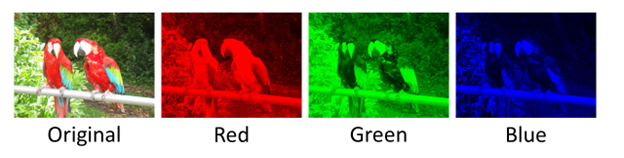
\includegraphics[width=0.8\textwidth]{Image/RGB.png}
            \captionof{figure}{Mô hình khối màu RGB}
        \end{column}
    \end{columns}
\end{frame}



\begin{frame}{Tại sao phải chuyển đổi không gian màu khi Fusion?}
    Trong fusion ảnh y tế, vấn đề lớn nhất là: \textbf{Không phải tất cả thông tin đều quan trọng như nhau}.
    \begin{itemize}
        \item \textbf{Intensity (Độ sáng)}: Chứa cấu trúc giải phẫu (xương, mô từ CT hoặc MRI).
        \item \textbf{Color (Màu sắc)}: Chứa thông tin chức năng (từ SPECT, PET).
    \end{itemize}
    
    \vspace{0.3cm}
    \textbf{Chiến lược Fusion chuẩn:}
    \begin{enumerate}
        \item Chuyển từ RGB sang các không gian \textbf{tách sáng vs màu}.
        \item Thực hiện Fusion trên kênh độ sáng (để tối ưu cấu trúc).
        \item Giữ nguyên hoặc xử lý riêng thông tin màu.
        \item Chuyển ngược về RGB để hiển thị.
    \end{enumerate}
\end{frame}

% ============================================================
\section{Không gian màu YUV}
% ============================================================

\begin{frame}{2. Không gian màu YUV}
    \textbf{Khái niệm:}
    \begin{itemize}
        \item Tách biệt Chiếu sáng (\textbf{Y}) và Hiệu màu (\textbf{U, V}).
    \end{itemize}
    
    \begin{block}{Công thức chuyển đổi (BT.601)}
    \begin{equation}
    \begin{aligned}
        Y &= 0.299R + 0.587G + 0.114B \\
        U &= -0.147R - 0.289G + 0.436B = 0.492(B - Y) \\
        V &= 0.615R - 0.515G - 0.100B = 0.877(R - Y)
    \end{aligned}
    \end{equation}
    \end{block}

    \vspace{0.2cm}
    \textbf{Vị trí trong Medical Fusion:}
    \begin{itemize}
        \item \textbf{Vị trí:} Ít dùng trong các Paper hiện đại (chủ yếu dùng trong video).
        \item \textbf{Thay thế:} Gần như bị thay thế hoàn toàn bởi YCbCr trong các nghiên cứu gần đây.
    \end{itemize}
\end{frame}

% ============================================================
\section{Không gian màu YCbCr}
% ============================================================

\begin{frame}{3. Không gian màu YCbCr (QUAN TRỌNG NHẤT)}
    \textbf{Lý thuyết cơ bản:}
    \begin{itemize}
        \item Phiên bản kỹ thuật số của YUV, dùng trong JPEG/MPEG.
        \item \textbf{Y (Luminance)}: Chứa toàn bộ các đặc trưng: \textbf{Edge (Cạnh), Texture (Vân), Structure (Cấu trúc)}.
        \item \textbf{Cb, Cr (Chroma)}: Chứa thông tin màu.
    \end{itemize}

    \begin{block}{Ma trận chuyển đổi (ITU-R BT.601)}
    \begin{equation*}
    \begin{bmatrix} Y \\ Cb \\ Cr \end{bmatrix} = \begin{bmatrix} 16 \\ 128 \\ 128 \end{bmatrix} + \begin{bmatrix} 65.481 & 128.553 & 24.966 \\ -37.797 & -74.203 & 112.000 \\ 112.000 & -93.786 & -18.214 \end{bmatrix} \begin{bmatrix} R \\ G \\ B \end{bmatrix}
    \end{equation*}
    \end{block}
\end{frame}

\begin{frame}{Quy trình chuẩn trong Image Fusion}
    \vspace{0.3cm}
    \textbf{Chiến lược thực hiện:}
    \begin{itemize}
        \item \textbf{CT/MRI} $\to$ Đưa thông tin cấu trúc dày đặc vào \textbf{kênh Y}.
        \item \textbf{PET/SPECT} $\to$ Màu sắc chức năng được giữ ở \textbf{Cb, Cr}.
        \item Xử lý: Tối ưu hóa kênh Y bằng các thuật toán phức tạp $\to$ Chuyển ngược RGB.
    \end{itemize}
\end{frame}

\begin{frame}{Tối ưu hóa Metric trên kênh Y}
    Fusion tốt thực chất là việc tối ưu hóa đúng \textbf{Y channel}. Đây là nơi các Paper tập trung sử dụng các chỉ số:
    \begin{columns}
        \begin{column}{0.5\textwidth}
            \begin{itemize}
                \item \textbf{QMI}: Chỉ số tương quan chất lượng.
                \item \textbf{SSIM}: Độ tương đồng cấu trúc.
                \item \textbf{Entropy}: Lượng tin thu được.
            \end{itemize}
        \end{column}
        \begin{column}{0.5\textwidth}
            \begin{block}{Insight cho nghiên cứu}
                Bản chất của các thuật toán Fusion hiện đại (CNN, Transformer) là tìm cách giữ được thông tin cấu trúc tốt nhất trên kênh Y mà không làm nhiễu thông tin màu ở Cb, Cr.
            \end{block}
        \end{column}
    \end{columns}
\end{frame}

% ============================================================
\section{Không gian màu HSY/HSV}
% ============================================================

\begin{frame}{4. Không gian màu HSY (Hue, Saturation, Luma)}
    \textbf{Khái niệm:}
    \begin{itemize}
        \item Là một biến thể của mô hình HSV, sử dụng giá trị \textbf{Luma (Y)} thay cho cường độ đơn giản.
        \item \textbf{H (Hue)}: Tông màu (Góc màu $0^\circ - 360^\circ$).
        \item \textbf{S (Saturation)}: Độ bão hòa (Độ thuần khiết).
        \item \textbf{Y (Luma)}: Độ sáng cảm nhận (tổng trọng số RGB).
    \end{itemize}
    \vspace{0.2cm}
    \begin{columns}
        \begin{column}{0.5\textwidth}
            \centering
            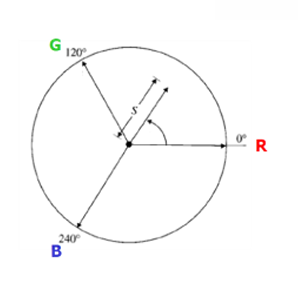
\includegraphics[width=0.8\textwidth]{Image/HSV.png}
        \end{column}
        \begin{column}{0.5\textwidth}
            \begin{itemize}
                \item Thay đổi \textbf{Y} giúp điều chỉnh độ sáng mà không làm biến đổi màu sắc.
                \item Thay đổi \textbf{S} giúp làm ảnh rực rỡ hơn hoặc chuyển về ảnh xám.
            \end{itemize}
        \end{column}
    \end{columns}
\end{frame}

\begin{frame}{HSV trong Medical Image Fusion}
    \textbf{Ý nghĩa y tế:}
    \begin{itemize}
        \item \textbf{H}: Loại màu; \textbf{S}: Độ bão hòa/đậm màu; \textbf{V}: Độ sáng.
    \end{itemize}

    \vspace{0.2cm}
    \textbf{Tại sao hạn chế trong Fusion?}
    \begin{itemize}
        \item \textbf{Tính không tuyến tính}: Các phép toán Fusion phức tạp khó áp dụng chính xác.
        \item \textbf{Grayscale}: CT/MRI thường là ảnh xám, không tận dụng được thế mạnh về Hue của HSV.
    \end{itemize}

    \vspace{0.2cm}
    \textbf{Ứng dụng thực tế:}
    \begin{itemize}
        \item Thường dùng trong \textbf{Segmentation} (phân đoạn) hoặc \textbf{Detection} (phát hiện vùng bệnh lý dựa trên sắc thái màu) hơn là dùng cho Fusion nghiêm túc.
    \end{itemize}
\end{frame}

% ============================================================
\section{Tổng kết}
% ============================================================

\begin{frame}{So sánh các hệ màu trong bài toán Fusion}
    \begin{table}
        \centering
        \small
        \renewcommand{\arraystretch}{1.2}
        \begin{tabular}{|l|c|c|c|}
            \hline
            \textbf{Tiêu chí} & \textbf{HSV} & \textbf{YCbCr} & \textbf{YUV} \\ \hline
            Phù hợp CT/MRI & \textcolor{red}{$\times$} & \textcolor{blue}{\checkmark} & \textcolor{orange}{!} \\ \hline
            Tách sáng/màu tốt & \textcolor{orange}{!} & \textcolor{blue}{\checkmark} & \textcolor{blue}{\checkmark} \\ \hline
            Dùng trong Paper & $\times$ & $\star\star\star\star$ & $\star$ \\ \hline
            Dễ optimize metric & $\times$ & \textcolor{blue}{\checkmark} & \textcolor{orange}{!} \\ \hline
        \end{tabular}
    \end{table}

    \vspace{0.4cm}
    \begin{block}{Kết luận}
        Để Fusion hiệu quả (giữ được Edge/Structure và tối ưu SSIM/Entropy), \textbf{YCbCr} là không gian màu quan trọng nhất cần tập trung trong các báo cáo khoa học.
    \end{block}
\end{frame}

% ============================================================
% Slide: Kết thúc
% ============================================================
\begin{frame}
    \centering
    \Huge \textcolor{hustred}{\textbf{CẢM ƠN THẦY VÀ CÁC BẠN}}
    \vspace{0.5cm}
    
    \Large \textbf{ĐÃ LẮNG NGHE!}
    
    \vspace{1cm}
    \normalsize
    \textit{Hỏi và đáp (Q\&A)}
\end{frame}

\end{document}
